\documentclass{article}
\usepackage{tikz} 
\usepackage{hyperref}
\usepackage[a4paper]{geometry}
\usepackage{fancyhdr}
\pagestyle{fancy}
\lhead{Energieniveauschemata}
\rhead{Dezember 2025}
\begin{document}
 
% TODO beispiel zeichnen 
\section{Energieniveauschemata}
Ein Energieniveauschema stellt die Energieniveaus eines Atoms dar.
 
\subsection{Aufbau} 
\begin{minipage}{\dimexpr\linewidth - 6cm}
Dieses hat die Bindungsenergie $E_B$ auf der $y$-Achse, nichts auf der $x$-Achse. Jedes Elekronenniveau wird durch eine horizontale Linie dargestellt, welche sowohl ein $n$ als auch eine eigene $E_B$ hat.
 
Ganz oben, mit $n \to \infty$ ist, per Definition, $E_B=0$. Weitere Energieniveaus werden weiter unten eingezeichnet, abhängig von ihrer $E_B$. Dabei ist $E_B(n)$ ein \hyperref[Das Linienspektrum von Wasserstoffatomen]{Linienspektrum} mit dem Endzustand von $\infty$ and einem Anfangszustand von $n$.
 
\subsection{Nutzen}
Die Differenz zwischen zwei Energieniveaus kann um einiges einfacher abgelesen werden. Diese stellt die absorbierte Energie bei einem Sprung eines Elektrons in ein höheres Niveau oder die Energie des emittierten Photons bei einem Sprung eines Elektrons in ein niedrigeres Niveau dar.
\end{minipage}
\hfill
\begin{minipage}{6cm}
 \center
 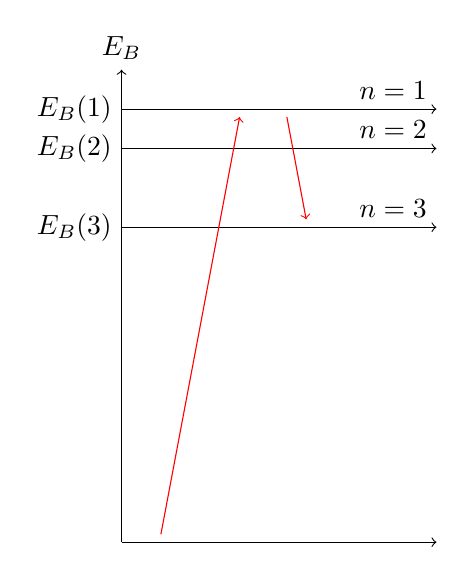
\begin{tikzpicture}
  \draw[->] (0, 0) -- (4, 0);
  \draw[->] (0, 0) -- (0, 6) node[above]{$E_B$};
  
  \draw[->] (0, 5.5) -- (4, 5.5) node [pos=0, left] {$E_B(1)$} node[above left]{$n=1$}; 
  \draw[->] (0, 5) -- (4, 5) node [pos=0, left] {$E_B(2)$} node[above left]{$n=2$};
  \draw[->] (0, 4) -- (4, 4) node [pos=0, left] {$E_B(3)$} node[above left]{$n=3$};
 
  \draw[->, red] (0.5, 0.1) -- (1.5, 5.4);
  \draw[->, red] (2.1, 5.4) -- ({2.1+(1.3/5.3)}, 4.1); 
 \end{tikzpicture}
\end{minipage} 
\end{document}